%CONFIGURACIÓN DEL DOCUMENTO Y HOJA
\documentclass[letterpaper, 12pt]{article}

%PAQUETES DEL TEMPLATE
\usepackage[inkscapelatex=false, inkscapearea=page]{svg}
\usepackage{fancybox}
\usepackage[utf8]{inputenc}
\usepackage{graphicx}
\usepackage{subcaption}
\usepackage{amsmath}
\usepackage{amsfonts}
\usepackage{amssymb}
\usepackage{eucal}
\usepackage[left=2.54cm, right=2.54cm, top=2.54cm, bottom=2.54cm]{geometry}
\usepackage[spanish, mexico]{babel}
\usepackage[colorlinks]{hyperref}
\usepackage{caption}
\usepackage{float}
\usepackage{siunitx}
\usepackage{color}
\usepackage{tikz}
\usepackage{minted}
\usepackage{circuitikz}

%CONFIGURACIONES
\svgpath{{./svgs/}}
\graphicspath{{./images/}}
\usemintedstyle{colorful}

\begin{document}
    \begin{center}
    \textsc{Universidad de Costa Rica} \\
    Escuela de Ingeniería Eléctrica \\
    TCU - 748 : Procesamiento de Voces \\
    \vspace{2mm}
    Luis Santiago Brenes Ruiz\\
    Y Wen Huang Shih
\end{center}

\vspace{-1mm}
\hrule height 0.8pt
\vspace{-2mm}

    \section{Uso de XTTSv2 en Kaggle}
    Para utilizar este TTS puede seguir los pasos en este documento o copiar el \href{https://www.kaggle.com/code/luissantiagobr/coquitts}{Notebook} directamente y editar las secciones necesarias como se indicará posteriormente.
    
    \subsection{Creación de un Notebook en Kaggle}
    Se utilizará Kaggle como entorno en la nube para entrenar/generar el modelo TTS ya que con el plan gratuito ofrece 30h semanales de uso en GPUs (2xT4 y P100) y persistencia en el almacenamiento (20GB).

    Para crear una cuenta puede dirigirse a la página oficial \href{https://www.kaggle.com}{Kaggle} y registrarse con sus datos.

    Una vez iniciada la sesión, desde la opción \textit{Create} (Figura \ref{fig:create}) puede abrir un Notebook nuevo que contendrá un celda por defecto como se observa en la Figura \ref{fig:notebook}
    \begin{figure}[h!]
        \centering
        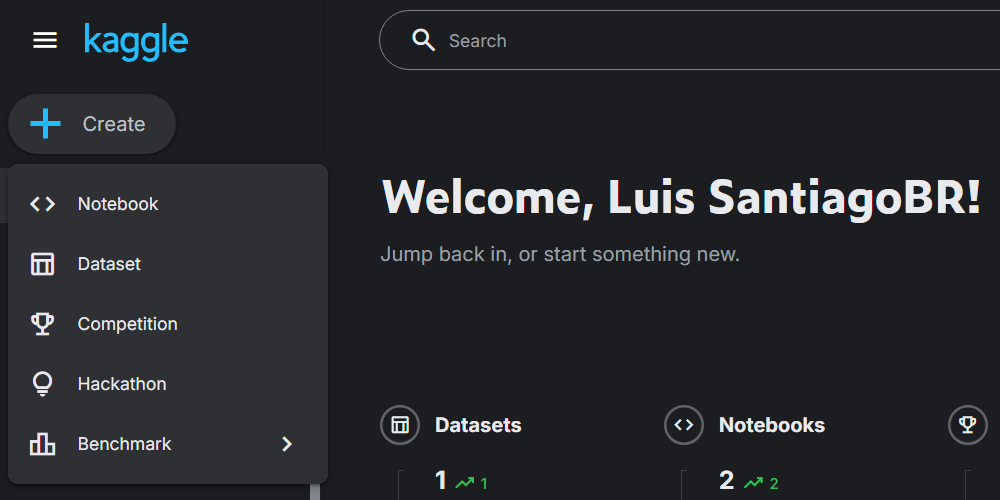
\includegraphics[width=0.45\linewidth]{crearNotebook.png}
        \caption{Menú \textit{Create}.}
        \label{fig:create}
    \end{figure}

    \begin{figure}[h!]
        \centering
        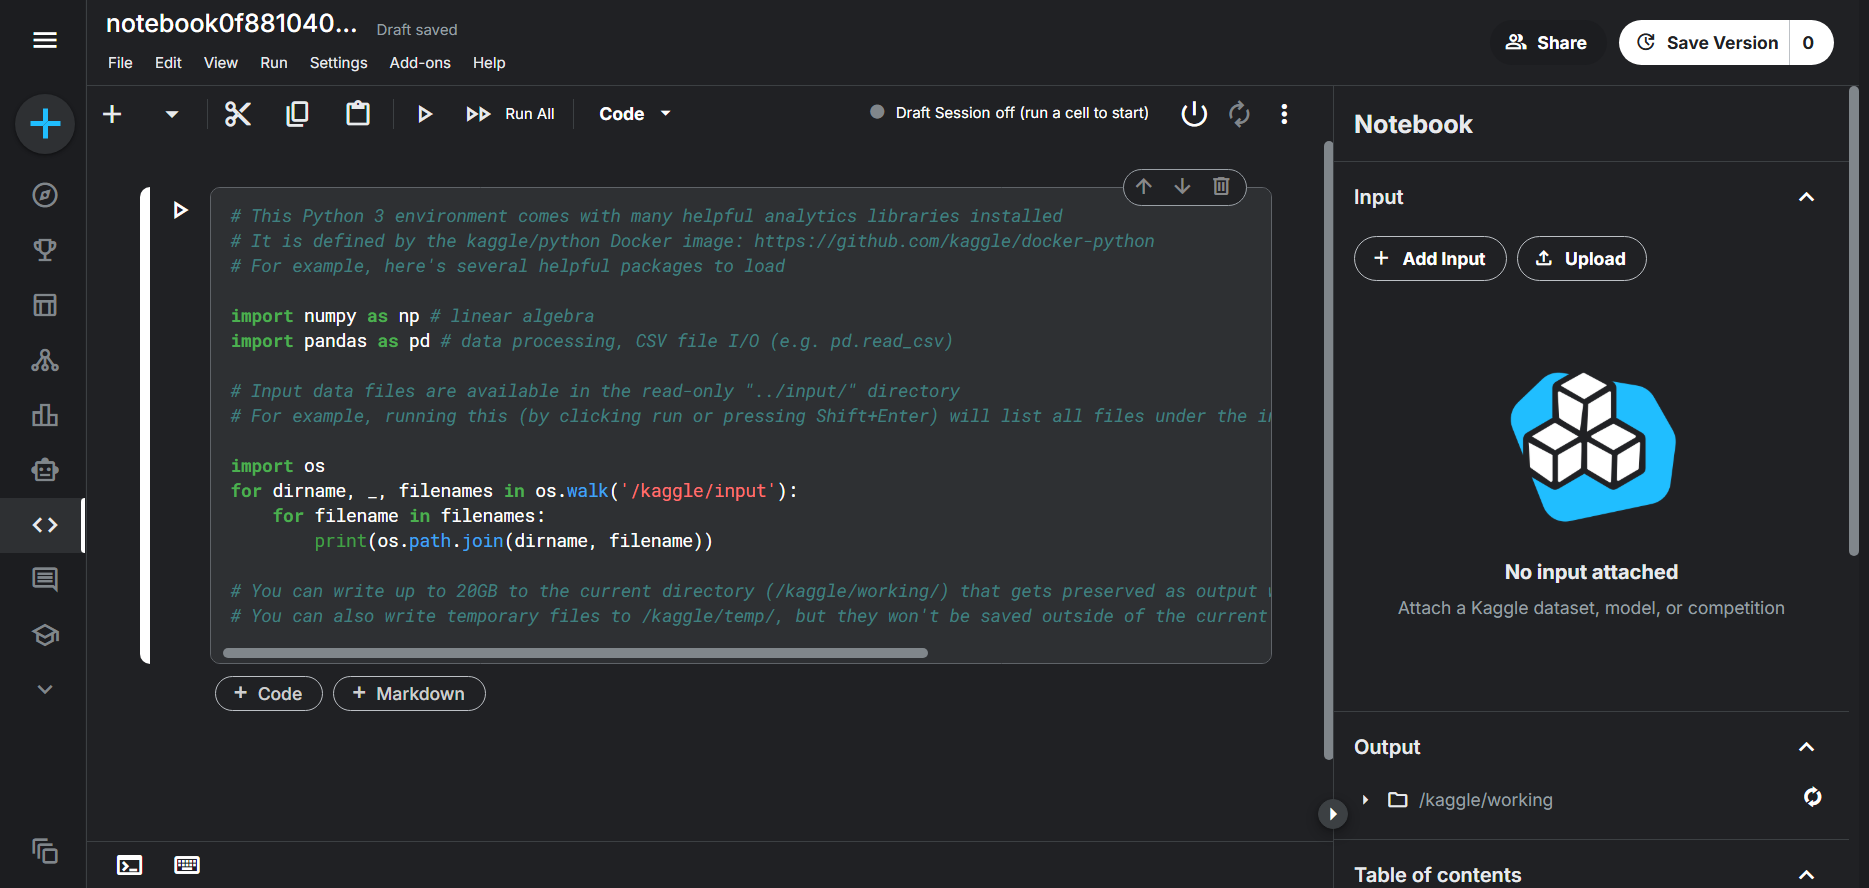
\includegraphics[width=0.75\linewidth]{notebook.png}
        \caption{Notebook nuevo en Kaggle.}
        \label{fig:notebook}
    \end{figure}

    \subsection{Subida de archivos a Kaggle}
    A diferencia de otras aplicaciones de, Kaggle solo permite subir archivos como un \textit{dataset} o \textit{model}. Para lograr esto en el menú desplegable de la derecha (Figura \ref{fig:notebook}) están las opciones \textit{Add Input} (para usar archivos ya cargados anteriormente por nosotros u otra persona) o \textit{Upload} (para nuevos archivos). 
    
    \textit{Nota:} Para el dataset es posible subir un archivo \texttt{.zip} el cual se descomprimirá automáticamente.

    Como recomendación para el entrenamiento del TTS, el dataset debe contener las grabaciones y transcripciones, de una voz seleccionada, nombradas por igual como se muestra en la Figura \ref{fig:dataset}.
    \begin{figure}[h!]
        \centering
        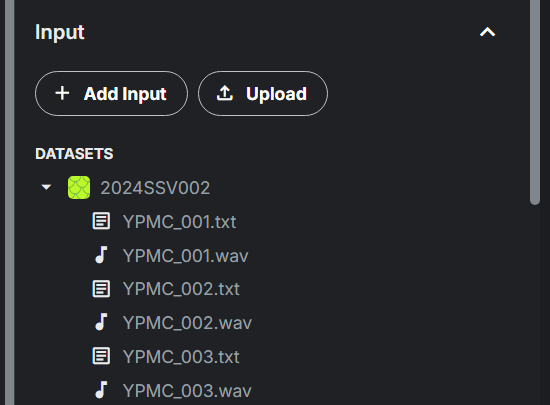
\includegraphics[width=0.35\linewidth]{dataset.png}
        \caption{Ejemplo de dataset para el TTS.}
        \label{fig:dataset}
    \end{figure}

    Para importar el modelo, utilice el repositorio de GitHub oficial: \url{https://github.com/idiap/coqui-ai-TTS} y la configuración de la Figura \ref{fig:repo}.
    \begin{figure}[h!]
        \centering
        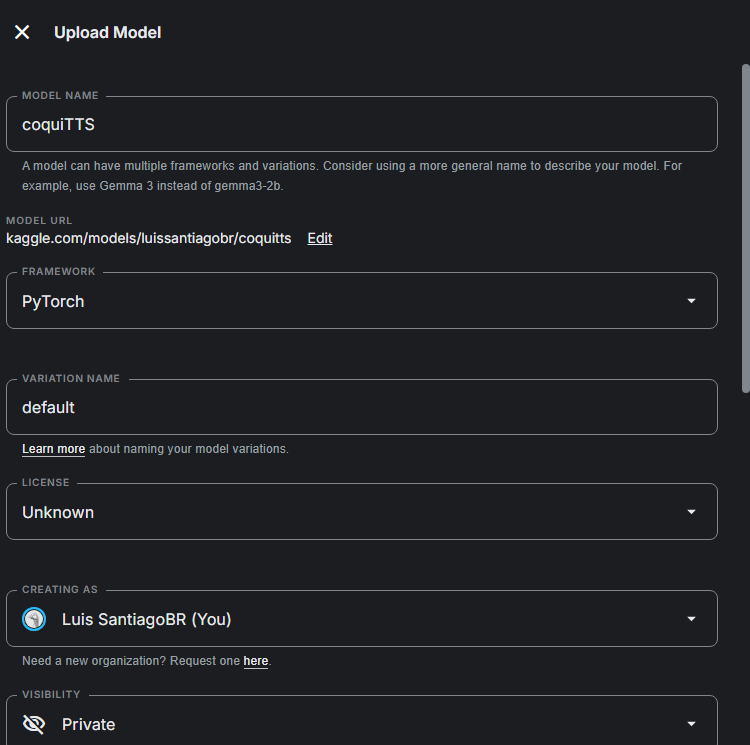
\includegraphics[width=0.45\linewidth]{repo.png}
        \caption{Datos sobre el repositorio.}
        \label{fig:repo}
    \end{figure}

    \subsection{Configuración de la sesión}
    Hay ajustes modificables en Kaggle, entre ellos el \textit{Acelerador} (CPU/None, GPU, TPU), la persistencia de almacenamiento y el uso de internet; para modificarlos, en el mismo menú de la derecha puede desplazarse hacia abajo hasta encontrar los ajustes de la Figura \ref{fig:sesion}.
    \begin{figure}[h!]
        \centering
        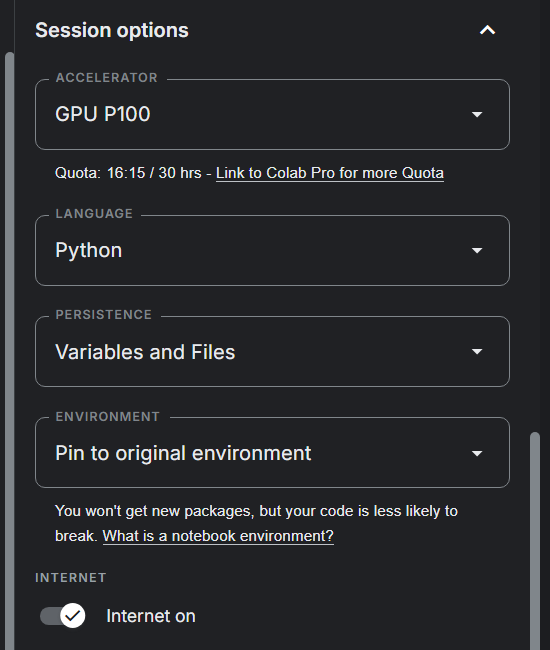
\includegraphics[width=0.45\linewidth]{sesion.png}
        \caption{Ajustes de la sesión.}
        \label{fig:sesion}
    \end{figure}

    Respecto al acelerador, este puede ser modificado posteriormente (lo que reiniciará el entorno). Para el modelo a usar (XTTS - coquiTTS), se recomienda usar \textbf{P100} como acelerador, ya que está optimizada para \textit{full precision FP32} a diferencia de \textit{T4}, que son mejores para entrenamientos con \textit{mixed precision FP16}.

    Con esto ya se encuentra configurado el entorno para iniciar una sesión (de máximo 12h seguidas) dando click al botón de ``encender''.

    \subsection{Uso de coquiTTS - XTTS}
    Primeramente se debe eliminar la celda por defecto, ya sea eliminando manualmente el contenido o creando una celda vacía y eliminando la original.

    \textbf{Celdas en Kaggle:}
    \begin{itemize}
        \item Todo lo escrito por defecto corresponde al lenguaje seleccionado (Python).
        \item Se puede utilizar \texttt{!comando} para ejecutar instrucciones en el terminal.
        \item Se puede utilizar \texttt{\%comando} para ejecutar instrucciones bash de una línea.
        \item Se puede utilizar \texttt{\%\%comando} para ejecutar instrucciones bash de varias líneas.
    \end{itemize}
    
    \subsubsection{Dependencias e Instalación}
    Antes de utilizar el TTS deben instalarse las dependencias requeridas, para ello se recomienda utilizar un entorno virtual con \texttt{uv} lo que evita algunos fallos por incompatibilidades.

    Los siguientes comandos deben ingresarse en una celda del Notebook o en celdas separadas:
    \begin{minted}[frame=lines, framesep=2mm, fontsize=\small]{cuda}
        !uv pip install torch torchaudio torchcodec --torch-backend=auto
        !uv pip install -e RUTA_MODEL
        !uv pip install -e RUTA_MODEL/[languages]
        !uv pip install transformers==5.0.0
        !uv pip install librosa soundfile
    \end{minted}
    
    \textit{Nota:} \texttt{RUTA\_MODEL} se obtiene presionando copiar en el modelo importado (Figura \ref{fig:ruta_model}).
    \begin{figure}[h!]
        \centering
        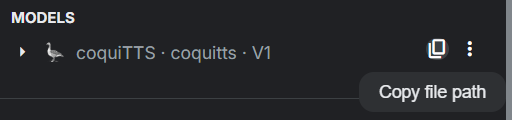
\includegraphics[width=0.45\linewidth]{rutaModel.png}
        \caption{Obtener la ruta del modelo.}
        \label{fig:ruta_model}
    \end{figure}

    Con esto ya se encuentra coquiTTS instalado con sus dependencias.

    \subsubsection{Preparar el dataset}
    En este documento se tomará de ejemplo el dataset con el formato recomendado anteriormente (grabaciones y transcripciones nombradas por igual).

    Para el entrenamiento se requieren las grabaciones en formato \texttt{.wav} y todas las transcripciones en un mismo archivo \texttt{.csv} siguiendo la estructura:
    \begin{minted}{text}
        dataset
          |
          +-- metadata.csv
          +-- wavs
                |
                +-- example1.wav
                +-- example2.wav
    \end{minted}

    Con el fin de automatizar el proceso de organización del dataset, copie en una celda el script \href{https://github.com/LSBR29/Procesamiento-de-Voces-TCU-748/blob/main/coquiTTS_Kaggle/generar_dataset.py}{\texttt{generar\_dataset.py}} y modifique cerca del final la línea que corresponde a la ruta del dataset original.
    \begin{minted}[fontsize=\small]{cuda}
        input_dir = "RUTA_DATASET"
    \end{minted}

    En caso de diferencias en los formatos de los archivos, puede modificar la extensión de los audios o el encoding de las transcripciones en las variables correspondientes.
    
    \subsubsection{Entrenamiento}
    Para el entrenamiento de XTTSv2 o cualquier otro modelo incluido en coquiTTS ya se proporciona un procedimiento en el repositorio original:
    \url{https://github.com/idiap/coqui-ai-TTS/blob/dev/recipes/ljspeech/xtts_v2/train_gpt_xtts.py}.

    Sin embargo requiere ciertas modificaciones, por lo que \href{https://github.com/LSBR29/Procesamiento-de-Voces-TCU-748/blob/main/coquiTTS_Kaggle/finetunning.py}{\texttt{finetunning.py}} ya se encuentra configurado para una voz en español.

    \textit{Importante:} Se debe modificar la ruta en la variable \texttt{SPEAKER\_REFERENCE} por una grabación existente en el dataset que está utilizando y debe establecer la transcripción de este audio en el parámetro \texttt{test\_sentences} de la variable \texttt{config} en la función \texttt{main()}:

    \begin{minted}[frame=lines, framesep=2mm, fontsize=\small]{python}
        def main():
            ...
            config = GPTTrainerConfig(
            ...
                test_sentences=[
                {
                    "text": "TRANSCRIPCION",
                    "speaker_wav": SPEAKER_REFERENCE,
                    "language": LANGUAGE,
                },
            )
        ],
    \end{minted}

    En ambos casos debe copiar en una celda las siguientes instrucciones para poder crear el archivo de entrenamiento.
    \begin{minted}[frame=lines, framesep=2mm, fontsize=\small]{cuda}
        %%writefile finetunning.py
        PEGAR AQUÍ EL SCRIPT CON LAS MODIFICACIONES
    \end{minted}

    Para ejecutar el entrenamiento, en una celda separada, luego de crear el archivo anterior, utilice el siguiente comando:
    \begin{minted}[fontsize=\small]{cuda}
        !CUDA_VISIBLE_DEVICES="0" python finetunning.py
    \end{minted}

    Una vez iniciado el proceso, este no se detendrá hasta que se le indique, lo recomendado es completar al menos 150 eppoch (épocas/iteraciones), también puede ejecutarlo hasta que los valores que se imprimen constantemente sobre el modelo varíen muy poco entre eppochs (AÚN POR DEFINIR).
    
    \subsubsection{Inferencia - Pruebas}
    Para las pruebas se requieren dos partes:
    \begin{itemize}
        \item Cargar el modelo según el entrenamiento.
        \item Generar y mostrar el audio.
    \end{itemize}

    La primera utiliza el script \href{https://github.com/LSBR29/Procesamiento-de-Voces-TCU-748/blob/main/coquiTTS_Kaggle/importar_modelo.py}{\texttt{importar\_modelo.py}} donde debe modificar las primeras 4 variables según los datos del entrenamiento.

    Para generar la voz utilice el script \href{https://github.com/LSBR29/Procesamiento-de-Voces-TCU-748/blob/main/coquiTTS_Kaggle/inferencia.py}{\texttt{inferencia.py}}, donde puede modificar el texto y los parámetros \texttt{temperature}, \texttt{top\_k}, \texttt{top\_p}, \texttt{repetition\_penalty} según considere necesario (AÚN POR DEFINIR).

    Estos códigos puede pegarlos directamente en una celda y ejecutarlos en cualquier momento tras el entrenamiento.

    En caso de querer reproducir el audio generado directamente en el notebook puede utilizar las instrucciones:
    \begin{minted}[frame=lines, framesep=2mm, fontsize=\small]{python}
        import IPython

        IPython.display.Audio("/kaggle/working/out.wav")
    \end{minted}

    \subsection{Nota Importante}
    Una vez el notebook contiene todas las celdas puede ejecutarlo directamente, sin embargo Kaggle no permite inactividad por más de 40min y cierra la sesión. Por ello, para el entrenamiento resulta conveniente presionar el botón \textit{Save Version} con la opción \textit{Save and Run} lo que ejecutará el notebook hasta que se indique lo contrario.

    \textbf{Documentación Original}\cite{coqui-original}: \url{https://docs.coqui.ai/en/latest/}
    
    \textbf{Documentación Comunidad}\cite{coqui-community}: \url{https://coqui-tts.readthedocs.io/en/latest/}
    
    
    \bibliographystyle{IEEEtran}
    \bibliography{biblio}
\end{document}